% Options for packages loaded elsewhere
\PassOptionsToPackage{unicode}{hyperref}
\PassOptionsToPackage{hyphens}{url}
%
\documentclass[
]{book}
\usepackage{amsmath,amssymb}
\usepackage{lmodern}
\usepackage{iftex}
\ifPDFTeX
  \usepackage[T1]{fontenc}
  \usepackage[utf8]{inputenc}
  \usepackage{textcomp} % provide euro and other symbols
\else % if luatex or xetex
  \usepackage{unicode-math}
  \defaultfontfeatures{Scale=MatchLowercase}
  \defaultfontfeatures[\rmfamily]{Ligatures=TeX,Scale=1}
\fi
% Use upquote if available, for straight quotes in verbatim environments
\IfFileExists{upquote.sty}{\usepackage{upquote}}{}
\IfFileExists{microtype.sty}{% use microtype if available
  \usepackage[]{microtype}
  \UseMicrotypeSet[protrusion]{basicmath} % disable protrusion for tt fonts
}{}
\makeatletter
\@ifundefined{KOMAClassName}{% if non-KOMA class
  \IfFileExists{parskip.sty}{%
    \usepackage{parskip}
  }{% else
    \setlength{\parindent}{0pt}
    \setlength{\parskip}{6pt plus 2pt minus 1pt}}
}{% if KOMA class
  \KOMAoptions{parskip=half}}
\makeatother
\usepackage{xcolor}
\usepackage{longtable,booktabs,array}
\usepackage{calc} % for calculating minipage widths
% Correct order of tables after \paragraph or \subparagraph
\usepackage{etoolbox}
\makeatletter
\patchcmd\longtable{\par}{\if@noskipsec\mbox{}\fi\par}{}{}
\makeatother
% Allow footnotes in longtable head/foot
\IfFileExists{footnotehyper.sty}{\usepackage{footnotehyper}}{\usepackage{footnote}}
\makesavenoteenv{longtable}
\usepackage{graphicx}
\makeatletter
\def\maxwidth{\ifdim\Gin@nat@width>\linewidth\linewidth\else\Gin@nat@width\fi}
\def\maxheight{\ifdim\Gin@nat@height>\textheight\textheight\else\Gin@nat@height\fi}
\makeatother
% Scale images if necessary, so that they will not overflow the page
% margins by default, and it is still possible to overwrite the defaults
% using explicit options in \includegraphics[width, height, ...]{}
\setkeys{Gin}{width=\maxwidth,height=\maxheight,keepaspectratio}
% Set default figure placement to htbp
\makeatletter
\def\fps@figure{htbp}
\makeatother
\setlength{\emergencystretch}{3em} % prevent overfull lines
\providecommand{\tightlist}{%
  \setlength{\itemsep}{0pt}\setlength{\parskip}{0pt}}
\setcounter{secnumdepth}{5}
\usepackage{booktabs}
\ifLuaTeX
  \usepackage{selnolig}  % disable illegal ligatures
\fi
\usepackage[]{natbib}
\bibliographystyle{apalike}
\IfFileExists{bookmark.sty}{\usepackage{bookmark}}{\usepackage{hyperref}}
\IfFileExists{xurl.sty}{\usepackage{xurl}}{} % add URL line breaks if available
\urlstyle{same} % disable monospaced font for URLs
\hypersetup{
  pdftitle={A Practitioner's Guide to Android Privacy},
  pdfauthor={Konrad Kollnig},
  hidelinks,
  pdfcreator={LaTeX via pandoc}}

\title{A Practitioner's Guide to Android Privacy}
\author{Konrad Kollnig}
\date{Version 2022-07-21}

\begin{document}
\maketitle

{
\setcounter{tocdepth}{1}
\tableofcontents
}
\hypertarget{preface}{%
\chapter*{Preface}\label{preface}}
\addcontentsline{toc}{chapter}{Preface}

\emph{This is a work-in-progress.}

Hello and welcome!

It's an honour that you found your way here. Privacy in apps is an important topic. But, what does this mean for me as an Android developer?

Surprisingly, there is very few information out there. This is true even though the General Data Protection Regulation (GDPR), Europe's flagship data protection law, was introduced in May 2018 -- quite a while back.

I, myself, have been an app developer for many, and spent hours browsing on the web to find out about how to comply.

`How do I do privacy in apps right?' is thus the question that this book seeks to address.

If you have any suggestions and feedback, then please reach out to \href{mailto:book@trackercontrol.org}{\nolinkurl{book@trackercontrol.org}}.


\includegraphics{images/by-nc-sa.png}\\
This online book is licensed under a \href{http://creativecommons.org/licenses/by-nc-sa/4.0/}{Creative Commons Attribution-NonCommercial-ShareAlike 4.0 International License}.

\hypertarget{about-the-author}{%
\chapter*{About the Author}\label{about-the-author}}
\addcontentsline{toc}{chapter}{About the Author}

Konrad is a current PhD student at the Computer Science Department of Oxford University. His research interest lies in data protection in smartphone apps and the regulation of tech companies. He is developing \emph{TrackerControl}, an Android app that shows you what companies track your app usage, and allows you to limit this. Further, he enjoys discussing all things technical on my blog. These experiences have motivated this short book.

\hypertarget{intro}{%
\chapter{Introduction}\label{intro}}

Have you ever worried about sharing an honest opinion with friend on WhatsApp, \href{https://www.wired.com/story/whatsapp-security-flaws-encryption-group-chats/}{or WhatsApp gaining access to the `encrypted' communications}? Have you worried about being listened to by the Facebook app, \href{https://www.newstatesman.com/science-tech/social-media/2018/03/testing-facebook-listens-your-conversations-adverts}{which it probably does not---they are just damn good at predicting your behaviour}? Or, ever drafted a Facebook post, which you ended up discarding, \href{https://slate.com/technology/2013/12/facebook-self-censorship-what-happens-to-the-posts-you-dont-publish.html}{which Facebook may retain regardless}? Have you worried about sending photos via Snapchat, \href{https://www.vice.com/en_us/article/xwnva7/snapchat-employees-abused-data-access-spy-on-users-snaplion}{or Snapchat staff having access to photos}?

If you confirm any of the above, you are probably not living freely in the digital world. Isn't this a bit frightening? Shouldn't our democratically elected government ensure the \href{https://oll.libertyfund.org/quotes/497}{protection is of our freedoms}, even in the digital world. Despite this, many of us feel surveilled. \href{https://www.theguardian.com/books/2019/feb/02/age-of-surveillance-capitalism-shoshana-zuboff-review}{Digitally surveilled}.

\hypertarget{what-is-privacy}{%
\section{What is privacy?}\label{what-is-privacy}}

Privacy is a highly individual concept. The privacy scholar Helen Nissenbaum characterised privacy as `contextual integrity'. This means that individuals try express themselves differently, depending on the \emph{context}, to protect their privacy. For instance, many people share different information with their boss at work than with their loves ones.

It is difficult to put this concept into software, though worth to remember. The aspect of privacy that this work focuses on is `data protection', a subject of much current debate. The European Union has strengthened the right to data protection in their 2018 General Data Protection Regulation (GDPR), a challenge and fear for app developers worldwide.

Data protection is rooted in the concept `informational self-determination'. This concept was first introduced by the \href{https://www.bundesverfassungsgericht.de/SharedDocs/Entscheidungen/EN/1983/12/rs19831215_1bvr020983en.html}{1983 landmark ruling} of the German Federal Constitutional Court. This highest German court concluded that

\begin{quote}
In the context of modern data processing, {[}human dignity, particularly the right to personal identity,{]} encompasses the protection of the individual against unlimited collection, storage, use and sharing of personal data. The fundamental right guarantees the authority conferred on the individual to, in principle, decide themselves on the disclosure and use of their personal data. Limitations of this right to ``\emph{informational self-determination}'' are only permissible if there is an overriding public interest.
\end{quote}

In other words, informational self-determination means that an individual should have control over the data that relates to him (such data is called \href{https://gdpr-info.eu/art-4-gdpr/}{`personal data' in GDPR}). As such, informational self-determination is similar to the concept of property, \href{https://leidenlawblog.nl/articles/privacy-and-property-do-you-really-own-your-personal-data}{yet not quite the same}.

\hypertarget{what-is-data}{%
\section{What is data?}\label{what-is-data}}

The most obvious form of data is what we actively share (Active Data). This is data from filling out forms about our personal details (whether online or offline), sharing pictures with friends, or sending emails. Most data however is not created directly by individuals, but rather created from them by a third party (Passive Data), by means such as observation, combination, or inference.

A ubiquitous example is \href{https://en.ryte.com/wiki/App_Tracking}{app tracking}, data collection from apps about usage behaviour. The collected data often includes which buttons you click, what purchases you make, and when and how often you use an app. Researchers from the University of Oxford found that \href{https://arxiv.org/pdf/1804.03603.pdf}{some 90\% of mobile apps could send such data to Google, some 40\% to Facebook}, and, most of the time, to numerous lesser known parties. The next chapter will cover this more in depth.

Passive Data is surprisingly valuable, and many previous calculations \href{https://ig.ft.com/how-much-is-your-personal-data-worth/}{underestimate its worth}. The business model of the online advertising industry revolves around this type of data. Only in 2018, Google generated \href{https://www.statista.com/statistics/266249/advertising-revenue-of-google/}{136.2bn US Dollars of revenue from advertising}. That's about 34 dollars of annual revenue from every one of the \href{https://wearesocial.com/blog/2018/01/global-digital-report-2018}{4bn global Internet users}, or 3 dollars per month.

\hypertarget{the-data-deal-would-you-sell-your-data}{%
\section{\texorpdfstring{The data deal\textbf{: }Would you sell your data?}{The data deal: Would you sell your data?}}\label{the-data-deal-would-you-sell-your-data}}

Suppose you were approached by a stranger in the street, offering you a deal: You'd install a little tool on your smartphone, that'd continuously share your visited websites with the stranger. The stranger may then do whatever he wants with your browsing history, but vows not to pass on any other directly identifying data such as name or email. In turn, you'd be given \emph{1 dollar per month}. That's about a third of what Google generates from every Internet user per month. Sounds good, doesn't it?

When making your decision, keep in mind that the calculations above did not factor in, amongst other aspects, the global differences in income. The median income per person in the United States lies \href{https://news.gallup.com/poll/166211/worldwide-median-household-income-000.aspx}{more than five times above} the global median. Even if you increase the monthly payment fivefold, the value of your data (not just the browsing history) is probably much higher than 5 dollars per month. These estimations only considered Google, not the whole advertising industry.

Further, data is usually collected irreversibly. Once data is collected, there are usually no means of getting it back (regardless of the legislation stipulating `informational self-determination'). Instead, our data is being \emph{stolen at scale}.

\hypertarget{so-what}{%
\section{So what?}\label{so-what}}

Does the ongoing, large-scale data theft cause harm? Cambridge Analytica used the \href{https://about.fb.com/news/2018/04/restricting-data-access/}{data of 87 million Facebook users} to sway elections. Surely, none of my data was used. And, if even so, I would certainly not be the one falling for the cheap tricks of a \href{https://www.theguardian.com/uk-news/2018/may/02/cambridge-analytica-closing-down-after-facebook-row-reports-say}{now defunct company}, right? Or worse, vote Trump.

A widely discussed issue of this data collection can now be witnessed in machine learning, whose use in industry is spreading. Machine learning systems are trained on data, that was generated from humans. Since humans are naturally biased in some way, the predictions of algorithms are subject to biases. Biases are often blamed on the underlying algorithms, but in fact, humans are at fault, in the design of algorithms, in the collection of data, and in the decision leading to unfettered data collection in the first place.

Biased data exhibits the problem that it may reinforce views and stereotypes of the past. This may not only lead to discrimination, but inhibit societal progress. It is often argued that data protection and thereby constraining data collection hampers economic progress. But, do we want to sacrifice societal progress? We need both.

\hypertarget{we-need-data-protection}{%
\section{We need data protection}\label{we-need-data-protection}}

Data is intangible, and the consequences of data collection are mostly invisible. Despite all legislative requirements, aiming to protect the informational self-determination of the individual, data continues to be collected, if not stolen, at scale. The collected data is incredibly valuable, yet collection mostly profits the data-collecting companies. Data collection is irreversible, and may impede societal progress, by reinforcing the stereotypes of the past. We, as a society, need data protection. And, app developer play a role in this.

\hypertarget{app-privacy}{%
\chapter{App Privacy}\label{app-privacy}}

This chapter provides a brief overview of the most important concepts of user privacy in apps. The concept of app tracking is discussed, as well as real-time bidding and the failed privacy tool `do not track', to show the helplessness of user, and the responsibility of developers to act.

\hypertarget{app-tracking}{%
\section{App Tracking}\label{app-tracking}}

In January 2020, the Norwegian Consumer Council, an NGO, published a report on collection and sharing of personal data in popular apps. The reassuring title: ``\href{https://fil.forbrukerradet.no/wp-content/uploads/2020/01/2020-01-14-out-of-control-final-version.pdf}{Out of Control: How Consumers Are Exploited by the Online Advertising Industry}''. On 186 pages, the researchers analysed the data practices of 10 popular Android apps. Amongst those apps: a children's app, a period tracker, and various dating apps. What they found was a blatant disregard for governing data protection legislation, notably the EU General Data Protection Regulation (GDPR).

\hypertarget{vulnerable-groups-at-risk}{%
\subsection{Vulnerable groups at risk}\label{vulnerable-groups-at-risk}}

\emph{Grindr}, a popular LGBTQ dating app, showed particularly troublesome data practices, for which reason it was singled out in the report. The app was found to share users' \emph{exact location, IP address, phone ID, age, and gender directly} with 18 third-party companies---including Google Crashlytics, Google Firebase, Tencent, Facebook, and Twitter's MoPub. To make matters worse, many of these companies reserve the right to pass this data on to many others in a ``cascading data sharing'' process. In consequence, potentially thousands of companies can get access to this private information.

In fact, the app was found to employ so-called real-time bidding, by which advertising space on a user's device is sold to interested advertisers in real-time. To facilitate these auctions, the app developer provides the interested advertisers with information about its users. I explain this business model in depth \textbf{a later chapter}.

\hypertarget{weve-been-there..}{%
\subsection{We've been there..}\label{weve-been-there..}}

Grindr has faced similar accusations in the past. Users can indicate on their profile whether they are HIV positive or negative, when they were last tested for STIs, and whether or not they take preventive medication against HIV. Previously, Grindr was found to share this medical information with two major analytics companies, only to analyse and improve app usage, they claim. This can put individuals at severe risk.

Homosexuality is illegal in more than 70 countries, in 13 of which it may be punished by death. Alone the use of Grindr, an indicator of sexual orientation, may motivate discrimination or prosecution. Even in countries without repressive legislative regimes, people are put at risk. Some people prefer not to disclose their sexual orientation publicly, and may face discrimination. Grindr only put an end to sharing health information following an official complaint by the Norwegian Consumer Council.

\hypertarget{were-all-affected.}{%
\subsection{We're all affected.}\label{were-all-affected.}}

Grindr maintains to ``operate with industry standard practices''. This is true. Similar extents of data sharing were found in many other (dating) apps. Tinder, a dating app, was found to share users' GPS location and ``target gender''---or data on sexual orientation. In addition to this information, OkCupid, another dating app, shared data on sexuality, political views and drug use with the analytics company Braze.

Concerning data practices were also found in the analysed children's and period tracker apps. One can thus very well describe the app ecosystem as ``out of control''. Overall, the bespoke report found widespread violations of data protection legislation. Data is shared, without the user's awareness, let alone consent.

\hypertarget{the-dangers-of-real-time-bidding}{%
\section{The dangers of real-time bidding}\label{the-dangers-of-real-time-bidding}}

On average, a person sees over 1 700 online ads per month. A significant proportion of these ads are disseminated using so-called \emph{real-time bidding} (RTB). Whilst the entire online advertising market has a size of 240bn USD, RTB only attracted 5bn USD in spending (1.8\%) in 2018. However, RTB is mainly used to sell low-quality ads on otherwise unused desktop and mobile display space. As a result, the proportion of RTB amongst the overall number of online ads may well be higher than 1.8\%. Unfortunately, there are no figures readily available, with RTB being a rather new technology. Spread and novelty of RTB motivate a closer look.

\begin{figure}
\centering
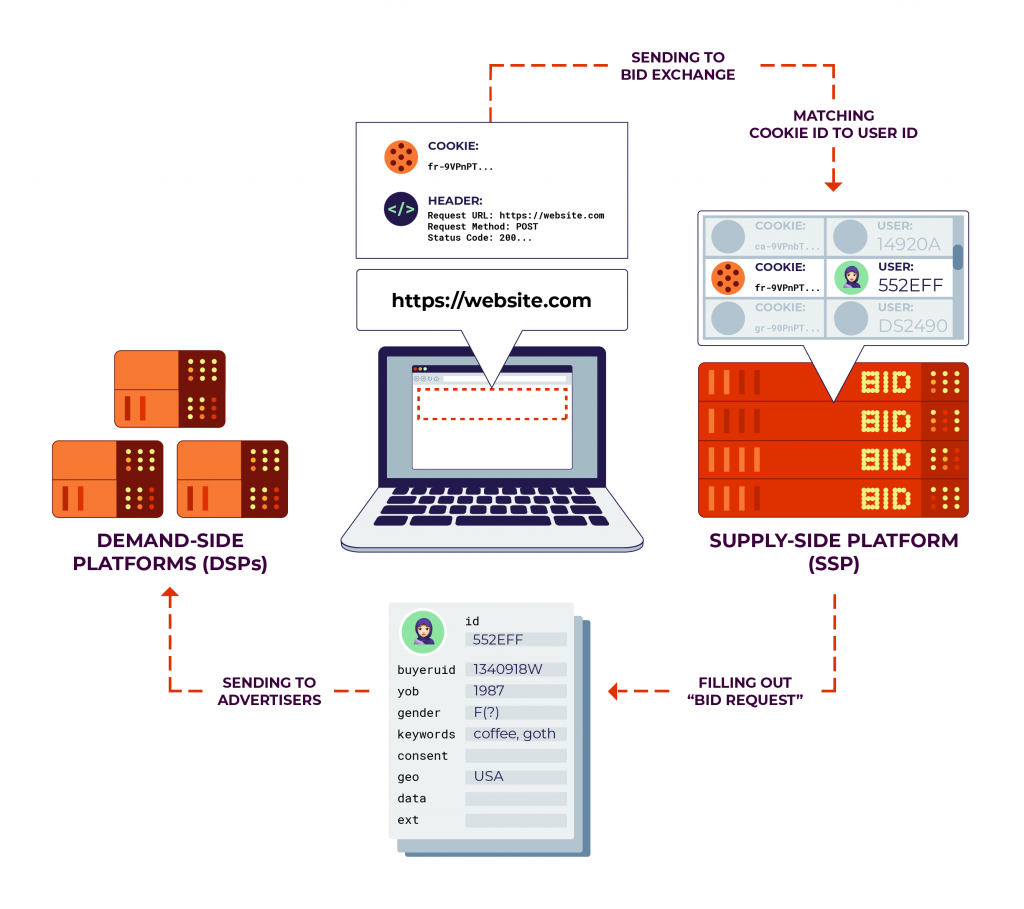
\includegraphics{images/real-time-bidding.png}
\caption{Supply-side platforms distribute ``bid requests'' with detailed information about the user to interested advertisers. \emph{Source: Electronic Frontier Foundation}}
\end{figure}

n RTB, advertising space on a user's device is sold via real-time auctions. These auctions are managed by \emph{ad exchanges}. Essentially, ad exchanges apply the concept of eBay to online advertising space. Prominent ad exchanges are Google's DoubleClick, Microsoft Advertising, and Twitter's MoPub.

The user (``supply side'') provides the advertising display space on their desktop or mobile device, whilst the advertiser (``demand side'') is interested in buying this display space. The auction proceeds as follows: The user's device requests an ad from an \emph{ad exchange} (``supply-side platform''), a platform for ad auctions. This request usually contains additional data, such as visited website, user identifiers, phone number, or location. The ad exchange may \emph{enrich the data} received from the user with further data, and then contact interested bidders (``bid request''). The bidders (``demand-side platforms'') receive this information about the user and may make a bid to purchase the offered advertising space on the user's device. Bidders usually have less than 100ms to respond, after which the auction ends. The highest-paying ad is shown to the user.

The whole process from requesting till serving an ad takes about 200ms.

Real-time bidding comes with severe privacy issues for the user. The real ``supply'' is the user data, according to which the ads are served. This user data is usually exposed to hundreds of advertisers, that can follow users around the internet and build comprehensive profiles. Moreover, this approach to online advertising relies to a large extent on inferences. Inferences are prone to false assumptions and may raise further issues, such as discrimination. Lastly, what is sold on ad exchanges is not only advertising space, but also the user's attention.

The questionable practices are currently being investigated by the UK Data Protection Regulator, the ICO, which has announced to \href{https://ico.org.uk/about-the-ico/news-and-events/news-and-blogs/2020/01/blog-adtech-the-reform-of-real-time-bidding-has-started/}{take further action} against advertising companies, which ``have their heads firmly in the sand''.

\textbf{Further reading:}

\begin{itemize}
\tightlist
\item
  Electronic Frontier Foundation: ``Behind the One-Way Mirror: A Deep Dive Into the Technology of Corporate Surveillance'', 2019, \url{https://www.eff.org/wp/behind-the-one-way-mirror}
\end{itemize}

\hypertarget{how-is-my-app-doing}{%
\section{How is my app doing?}\label{how-is-my-app-doing}}

If you're curious now how your app is doing, look no further! There are a couple of tools online that help provide some insights into the privacy of Android apps.

\hypertarget{exodus-privacy}{%
\subsection{Exodus Privacy}\label{exodus-privacy}}

\begin{figure}
\centering
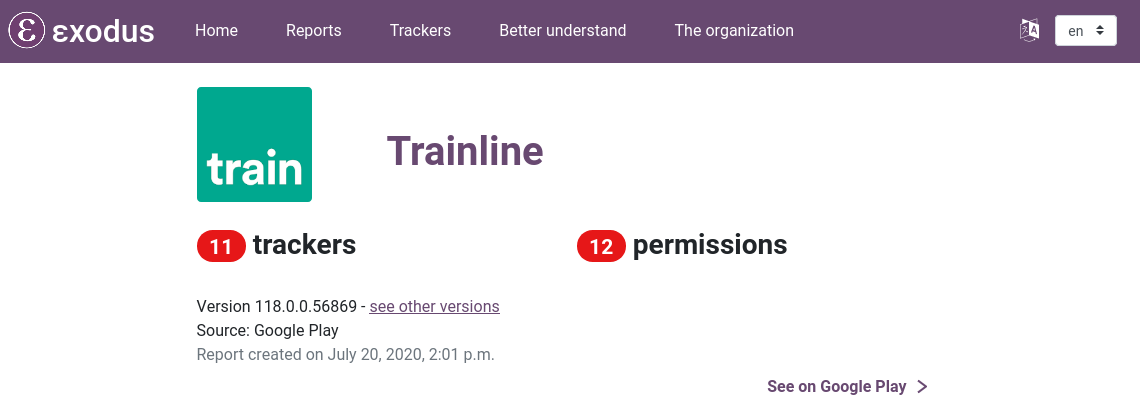
\includegraphics{images/exodus.png}
\caption{exodus}
\end{figure}

\href{https://reports.exodus-privacy.eu.org/en/}{Exodus Privacy} is an ambitious project by a group around French app privacy advocates. This group tries to create a database of the whole app tracking ecosystem. They provide the tools to analyse apps for privacy aspects, cultivate a database of relevant privacy characteristics, and regularly scan the most popular Android apps for privacy aspects with their tools.

At the time of writing, their database comprises 304 tracker companies, with which apps have been found to share data. They have analysed 76~530 Android apps. You can \href{https://reports.exodus-privacy.eu.org/en/reports/}{search for your app on their website}, or initiate an analysis if not yet on their database.

If you prefer to keep the results of the analysis private, all tools are open-source, and can be run locally. You can find the analysis tool for your use \href{https://github.com/Exodus-Privacy/exodus-standalone}{on GitHub}. It's super simple to use.

\hypertarget{appcensus}{%
\subsection{AppCensus}\label{appcensus}}

\begin{figure}
\centering
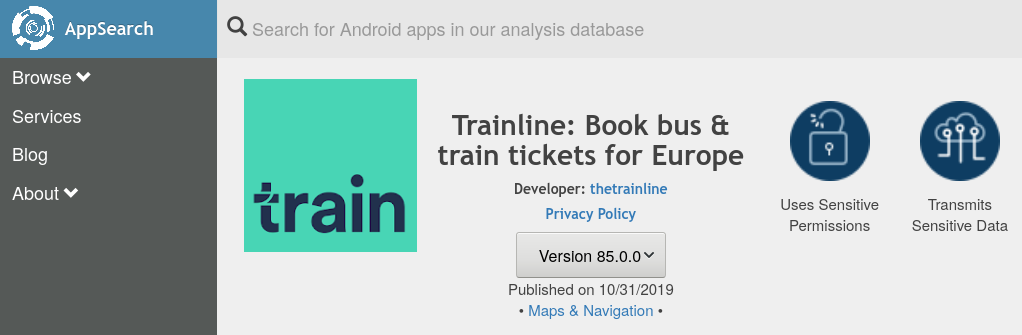
\includegraphics{images/app_census.png}
\caption{app\_census}
\end{figure}

\href{https://search.appcensus.io/}{AppCensus.io} is another ambitious project to scrutinise the privacy of Android apps. Compare to Exodus, these researchers focus more on run-time behaviour on apps, rather than tracking capabilities of apps. As a result, their database provides very detailed insights into actual app behaviour. This data is obtained by running the apps on actual phones (they claim).

Unfortunately, AppCensus is a commercial project, and none of their tools has been published. This means their analysis tools be used by non-affiliated app developers.

\hypertarget{trackercontrol}{%
\subsection{TrackerControl}\label{trackercontrol}}

I, myself, am developing a tool -- called TrackerControl -- to provide insights into app privacy. TrackerControl allows users to monitor and control the widespread, ongoing, hidden data collection in mobile apps about user behaviour (`tracking'). To detect tracking, TrackerControl checks all network traffic against the \emph{Disconnect blocklist}, used and trusted by the Mozilla Firefox browser. Additionally, our in-house blocklist is used, created \emph{from analysing \textasciitilde1 000 000 apps}!

This approach

\begin{itemize}
\tightlist
\item
  reveals the companies behind tracking,
\item
  allows to block tracking selectively, and
\item
  exposes the purposes of tracking, such as analytics or advertising.
\end{itemize}

The app also aims to educate about \emph{your rights} under Data Protection Law, such the EU General Data Protection Regulation (GDPR).

Under the hood, TrackerControl uses Android's VPN functionality, to analyse apps' network communications \emph{locally on the Android device}. This is accomplished through a local VPN server, to enable network traffic analysis by TrackerControl. This VPN layer is adopted from NetGuard, a popular Android firewall. Like NetGuard, TrackerControl additionally allows you to block certain DNS requests, e.g.~to advertising companies, and to retrieve a log of all network communications. No external VPN server is used, to keep your data safe!

TrackerControl can be downloaded \href{https://github.com/OxfordHCC/tracker-control-android/releases}{directly from GitHub}, including automatic checks for updates. Alternatively, the app is available on \href{https://f-droid.org/packages/net.kollnig.missioncontrol.fdroid}{F-Droid}, the most popular open-source Android app store. It is also available on the \href{https://apt.izzysoft.de/fdroid/index/apk/net.kollnig.missioncontrol}{IzzyOnDroid} F-Droid Repository. A feature-reduced version is also available on \href{https://play.google.com/store/apps/details?id=net.kollnig.missioncontrol.play}{Google Play}.

\hypertarget{shouldnt-users-act-on-privacy-rather-than-developers}{%
\section{Shouldn't users act on privacy, rather than developers?}\label{shouldnt-users-act-on-privacy-rather-than-developers}}

User privacy is widely neglected. Why then, should you as a developer do things differently? What difference would it make? And then, doesn't the obligation lie with users to take care of their privacy? Unfortunately, users have little choice over how their data is treated, particularly in mobile. The challenge is to strike a balance between users, and those interested in data. Past attempts have failed.

The most notable past attempt was the idea of a ``Do-Not-Track'' (DNT) setting, emerged in 2009. This system gives users a simple choice to reject and accept online tracking on websites. Despite great ambitions, DNT has failed, whilst the practice of tracking continues. I want to explore with you why, but also how DNT has managed to change user privacy for the better.

\hypertarget{history-of-implementation}{%
\subsection{History of implementation}\label{history-of-implementation}}

After its first proposal in 2009, the Federal Trade Commission (FTC), which regulates privacy in the US, quickly picked up the idea of DNT. The FTC expressed their backing for DNT as an \href{https://www.wired.com/2010/12/ftc-do-not-track/}{effective alternative to failed industry self-regulation}. At the time, the tracking industry was offering a central website to users, to opt-out by setting the right cookies. Since this was unreliable and created further privacy risks, the FTC regarded DNT as a more robust solution to restrict tracking, not relying on cookies.

DNT works by the user's browser sending a binary value to every website visited. This value, of whether or not tracking is allowed, is sent to a website in the request header, alongside other information such as requested URL. The W3C, responsible for standards on the Internet, started to work towards a common standard from 2011. By 2012, all major browsers had implemented DNT. In this implementation, the user could choose from the browser settings to enable DNT.

\hypertarget{reasons-for-failure}{%
\subsection{Reasons for failure}\label{reasons-for-failure}}

The weakest point of DNT is its reliance on the tracking industry. Implementation in all major browsers is not enough. Websites using tracking must also respect the user's DNT setting. Also, it is not clear what a DNT signal to a website actually means. Must all data collection on a website be stopped? Are certain types of data collection, such as analytics, still allowed?

With a lack of regulatory obligations and standardisation, very few services ever respected DNT. The search giant and largest online advertising company, Google, never implemented support for DNT on their websites or in their analytics tools. Similarly, other big tech companies, including Facebook and Twitter, simply ignore the DNT signal. Instead, browsers were \href{https://gizmodo.com/do-not-track-the-privacy-tool-used-by-millions-of-peop-1828868324}{``just screaming for privacy into a void''}, as expressed by the tech magazine \emph{Gizmodo}.

Worryingly, DNT can have unexpected, negative implications for user privacy. Since only a small minority of users ever used the setting, DNT can be used to identify users. This technique called ``browser fingerprinting'' creates a unique user identify from your individual browser characteristics. If only enough characteristics of your web browser, such as your DNT setting, are combined, this can be used to identify you. You can find out how unique your browser is with INRIA's \href{https://amiunique.org/}{amiunique.org} service.

Since there were no sufficient \href{https://github.com/w3c/dnt/commit/5d85d6c3d116b5eb29fddc69352a77d87dfd2310}{``indications of planned support among user agents, third parties, and the ecosystem at large''}, the W3C stopped their efforts in January 2019. The following month, \href{https://www.fastcompany.com/90308068/how-the-tragic-death-of-do-not-track-ruined-the-web-for-everyone}{Apple removed support for DNT} from their Safari browser.

\hypertarget{privacy-a-binary-setting}{%
\subsection{Privacy, a binary setting?}\label{privacy-a-binary-setting}}

Whilst it is easy to blame the failure of DNT on the advertising industry, the issue is arguably more complex than it first seems. Many content creators online, including news outlets, rely on advertising revenue, and so an outright ban of tracking would be devastating for their business models. A black and white setting does not give user a real choice to allow certain types of information sharing. Much controversy was caused by Microsoft choosing to enable DNT by default in their Internet Explorer 10 on Windows 8. Other browsers had left it to their users to find the DNT setting in the depth of browser configurations.

The debate around DNT foremost took place in the US, which lacks a federal privacy law. By contrast, online tracking has long been on thin ice in the EU. According to EU data protection legislation, as little data as possible should be collected (\emph{data minimisation}). Online tracking is widely considered to not be essential and explicit user consent is required. EU Internet users see more consent banners than US ones, given the lack of an established opt-out solution such as DNT.

\hypertarget{the-spirit-of-dnt-lives-on}{%
\subsection{The spirit of DNT lives on}\label{the-spirit-of-dnt-lives-on}}

Despite the failure of DNT, it managed to change user privacy permanently for the better. Browser manufacturers have realised that a consensual implementation of user privacy without the explicit cooperation of tracking companies will be difficult--unless there are incentives to do so. Instead, Safari and Firefox now resort to \emph{tracker blocking}, that does not rely on tracking companies. Whilst ad blocking has been widely popular for some time, these new anti-tracking solutions do not primarily aim to block ads, but rather to protect user privacy.

Privacy is more complex than the click of a button, and many website owners rely on the evaluation of user behaviour. On both Safari and Firebox, the user can choose different levels of blocking, and disable tracking protection for every site visited. This avoids problems with website breakage due to blocking, affords users higher granularity than previous solutions, and aims for more fairness towards website owners.

\hypertarget{tracking-continues-whats-next-for-user-privacy}{%
\subsection{Tracking continues, what's next for user privacy?}\label{tracking-continues-whats-next-for-user-privacy}}

Google Chrome takes the opposite direction than Safari and Firefox. Instead of pushing for increased tracking protection, the company is currently reworking the browser APIs, upon which current ad and tracking blockers rely. This will restrict the number of URLs that can be monitored by browser extensions. This monitoring is currently used to block the connections to known tracker URLs. The official reason for this change is increased performance. Critics expect a profound impediment to current ad and tracking blockers.

Changes to Google Chrome have a large reach. Chrome leads the browser market, being \href{https://gs.statcounter.com/browser-market-share/desktop/worldwide}{used by 68\% of desktop users}. Safari and Firefox only attract 9\% of users each. It is known that Google relies on advertising and data collection. They have a natural interest in limiting ad and tracker blockers. What might be less known to browser users is that the choice of browser is also a choice of privacy.

Overall, this highlights how DNT has failed, but has motivated new solutions against tracking. It also underlines that privacy cannot be taken for granted in the 21st century. We will need to continue the debate, and to seek innovative solutions around user privacy.

\hypertarget{legal-stuff}{%
\chapter{Legal Stuff}\label{legal-stuff}}

This chapter shall briefly summarise \emph{your legal obligations} as an app developer, under EU Data Protection Legislation (GDPR). This shall cover the most important buts, when pushling apps \emph{in non-legal terms}. Note that this is no no legal advice, only an app developer's attempt to make data protection more understandable.

You must respect the rules of GDPR, if you have app users from the European Union. This will almost always be the case. Usually, you are responsible for \emph{all} data collected through your app. GDPR protects personal data, which is data relating to individuals. This may include device data, pseudonyms, user identifiers, advertising identifiers, (dynamic) IP addresses, and postcodes, especially in combination with other data. For these reasons, it is usually not possible to make personal data non-personal. Almost all data collected from apps is personal, and requires careful protection.

You are also responsible for personal data collected from your app for third-party services, such as advertising, analytics, or crash reporting services. For instance, this means that you are even responsible for data, that is collected during the use of \emph{Google Firebase Analytics} or \emph{Crashlytics} -- even if you never see the raw data.

\textbf{Ask for consent}

You can only use most third-party services, including Firebase Analytics, after the user has agreed to this practice.

\emph{iOS:} According the Apple's terms, you should ask for user consent, before you or your third-parties collect \emph{any data}, no matter if personal and non-personal.

\emph{Android:} According to Google's terms, if you process sensitive data (e.g.~health-related), or process data in unexpected ways, do tell the user in a clear manner and ask for his \emph{consent} (no pre-ticked boxes allowed). Google also states that the use of some of their services, such as Firebase Analytics, needs explicit user consent.

\textbf{Always provide a privacy policy.} Provide a privacy policy on the app store and within the app. You may want to use one of the privacy policy generators, such as \href{https://gdpr4devs.com/iubenda.com}{iubenda.com}. Make sure it discloses the data collection of you and your third-parties adequately.

\textbf{Risk evaluation and documentation.} GDPR acknowledges that there will never be full protection of personal data. Instead, it encourages a risk-based approach, that is, seriously analysing the possible risks to data protection and taking appropriate data protection measures. If you can prove that you took all appropriate measures, there is no need to be overly afraid of high fines.

Make sure that you can provide such proof, by \emph{documenting all data protection considerations, decisions, and actions}.

\textbf{Reasonable data collection.} You and your third-parties may only collect personal data reasonably, that is, only for the purposes stated in your privacy policy (purpose limitation) and restricted to what is necessary for the stated purposes (data minimisation).

Furthermore:

\begin{itemize}
\tightlist
\item
  At best, use at most one third-party service for one purpose, that is, at most one advertising, analytics, and crash reporting service.
\item
  Check with every app release, if you can reduce data collection or remove any third-party services.
\item
  Verify the default settings of your third-party services (on-device and server-wise), since third-parties have an interest in collecting ever more data. Only activate third-party services, once user consent is established. More information can be found in the Appendix below.
\item
  If your app is aimed at \emph{children}, do not employ any third-party services. It's not good practice, and a violation of Apple's terms.
\end{itemize}

\textbf{Handling user requests.} The GDPR entitles users to manage (e.g.~access, delete, correct) any data about them. You can implement these user rights directly in software, which would show your efforts towards GDPR compliance. Yet, taking requests via email seriously is just as fine. You have one month to respond to user requests. This response may either address the request, or, for complex user requests, request an extension for a further 2 months.

\textbf{Security measures and data breaches.} Take the standard measures for security, such as HTTPS communications, salted passwords, validation of user inputs. Apple (\href{https://developer.apple.com/documentation/security}{here} and \href{https://developer.apple.com/library/archive/documentation/Security/Conceptual/SecureCodingGuide}{here}) and \href{https://developer.android.com/training/articles/security-tips}{Google} provide comprehensive guidance on this. Try to remove identifiable information whenever possible, through pseudonymisation or anonymisation. If you experience a \emph{personal data breach}, you must notify \href{https://edpb.europa.eu/about-edpb/board/members}{the data protection authority} within 72 hours, plus the individuals in case of high risk.

\textbf{Consent for third-party services.} If you use third-party services, the user must be asked for consent in almost all circumstances. This consent must be sought before the third-party service is activated and begins to share data. Beyond consent, the Appendix below provides more detail on the correct implementation of the most widely used third-party services.

\textbf{Closing remarks.} By implementing these measures, you should come an important step closer to compliance with GDPR. Additionally, you should consult the guidelines of an EU data protection authority. The British Data Protection Authority, called ICO, provides \href{https://ico.org.uk/for-organisations/}{excellent guidance} on data protection.

\hypertarget{sources}{%
\section{Sources}\label{sources}}

\begin{itemize}
\tightlist
\item
  European Parliament and Council: ``Regulation 2016/679 (General Data Protection Regulation)''
\item
  Article 29 Data Protection Working Party: ``Opinion 02/2013 on apps on smart devices''
\item
  Google LLC: ``Google Play Developer Distribution Agreement'' (version 15 April 2019)
\item
  Google LLC: ``Google Play Developer Program Policies'' (accessed 20 June 2019)
\item
  Apple Inc: ``Apple Developer Program License Agreement'' (accessed 20 June 2019)
\item
  Apple Inc: ``App Store Review Guidelines'' (version 3 June 2019)
\item
  The documentation of the top 18 third-party services in apps, from 10 different companies.
\end{itemize}

\hypertarget{methodology-behind-these-guidelines}{%
\section{Methodology behind these guidelines}\label{methodology-behind-these-guidelines}}

These legal guidelines shall cover the fundamentals of GDPR. These are 1) the key concepts, 2) user rights, and 3) principles and obligations. Legal terminology shall be avoided, to make the guidelines understandable without expert knowledge.

\hypertarget{key-concepts}{%
\subsection{Key concepts}\label{key-concepts}}

The app developer shall be made aware of what GDPR protects, that is, \emph{personal data}. Personal data is relevant for the developer, being responsible for its protection as the \emph{data controller}. There has been much public attention on the \emph{high penalties}, introduced by GDPR. The risk of such penalties is low, if the developer follows a \emph{risk-based approach} to data protection, as advocated by GDPR.

\hypertarget{user-rights}{%
\subsection{User rights}\label{user-rights}}

Not all developers will be aware of the profound rights, that GDPR grants to users. These shall be mentioned.

\hypertarget{principles-and-obligations}{%
\subsection{Principles and obligations}\label{principles-and-obligations}}

The rest of the document shall cover the seven principles of GDPR, that the developer must follow as data controller:

\begin{itemize}
\tightlist
\item
  Lawfulness, fairness and transparency,
\item
  Purpose limitation,
\item
  Data minimisation,
\item
  Accuracy,
\item
  Storage limitation,
\item
  Security, and
\item
  Accountability.
\end{itemize}

To cover the first principle, ``lawfulness, fairness and transparency'', the most important step is the provision of an adequate \emph{privacy policy}. There exist rich online resources, which shall be mentioned.

For simplicity, the principles ``purpose limitation'', ``data minimisation'', ``accuracy'', and ``storage limitation'' shall be summarised as \emph{reasonable data collection}. The term ``reasonable'' is similarly used in the GDPR and occurs widely across the GDPR document, 52 times.

Regarding data collection, the further provisions of the platform providers, Apple and Google, shall be added.

The remaining principles of ``security'' and ``accountability'' shall be mentioned. Regarding security, Apple and Google provide support documents, that shall be linked.

\hypertarget{technical-implementation-work-in-progress}{%
\chapter{Technical Implementation (work-in-progress)}\label{technical-implementation-work-in-progress}}

As a developer, you often depend on the use of third-party tools, such as Google Analytics or AdMob. This is completely fine, and nothing to be ashamed of. However, you probably have thought much about user privacy. So, this chapter shall tell you about some best practices.

\hypertarget{consent}{%
\section{Consent}\label{consent}}

If you use third-party tools, it is best practice to give users an option over this data sharing. Indeed, under EU law, this will often be a legal requirement.

When you implement consent in apps, it is important that you ask for consent \emph{before you initialise} most of your third-party tools. This is because EU law (the ePrivacy Directive in Article 5(3)) requires you to seek consent before you access or store information in on user's device, unless such is strictly necessary. Analytics or ads are not usually strictly necessary and thus need consent.

When asking for consent, make sure you make it for end-users as easy to decline as it is to accept. This means that you should use the same colour for both options and also use neutral (and not leading) language for these options.

A good overview of how to implement consent is provided by the French data protection authority at \url{https://design.cnil.fr/en/concepts/consent/}.

In implementing consent, you might be playing with the idea of using a consent management platform (CMP). While some CMPs have good features, they can also introduce additional compliance risks. This is because CMPs often involve a significant amount of additional data collection before consent is given. This is why it is better, if you can, to implement the consent flow yourself. This is not complicated. Sample consent implementation for consent on Android can be found on GitHub. For example:

\begin{itemize}
\tightlist
\item
  \url{https://github.com/kasnder/app-consent-android}
\item
  \url{https://github.com/gdprsdk/android-gdpr-library}
\item
  \url{https://github.com/DavidEdwards/GDPRConsent}
\end{itemize}

\hypertarget{using-popular-third-party-services-right}{%
\section{Using popular third-party services right}\label{using-popular-third-party-services-right}}

At best, you should use as few third-party services as possible. If you do, you have some options to improve user privacy.

\textbf{Adjust}. Once the Adjust SDK is enabled in your app, data sharing takes place, notably of device events. User consent should be established before enabling this SDK. It stands out that Adjust integrates the GDPR \emph{right to deletion} into their SDK. This could be implemented in your app, to show your efforts to comply with GDPR.

\emph{More info:} \url{https://github.com/adjust/sdks}

\textbf{AppLovin}. For EU users, AppLovin requires consent to be passed on programmatically. If consent is given, the Advertising ID and IP address will be sent to advertising partners, otherwise only a country code. Once loaded at runtime, AppLovin automatically receives the information that the app was installed.

\emph{More info:} \url{https://www.applovin.com/gdprfaqs/}

\textbf{AppsFlyer}. The service collects the Advertising ID and a unique AppsFlyer user ID from the first app start. User consent should be established before activating this service. If the Advertising ID cannot be accessed, permanent identifiers, notably the device's IMEI, are shared with AppsFlyer, unless programmatically disabled. Such permanent identifiers are highly critical from a data protection standpoint. This practice should be communicated transparently to the user, if not disabled.

\emph{More info:} \url{https://support.appsflyer.com/hc/en-us/articles/360001422989}

\textbf{Facebook SDK}. From the first app start, the Facebook SDK collects device information and events (app installation, app start, in-app purchases), unless programmatically disabled. User consent should be established before activating this SDK. Facebook serves no advertising, if the user limits interest-based ads from the device settings.

\emph{More info:} \url{https://developers.facebook.com/docs/app-events/best-practices/gdpr-compliance}

\textbf{Flurry}. For ads, this service provides a complicated mechanism to establish a user consent. Since legally required for many advertising services, you may want to consider easier, alternative approaches to establish valid user consent. Unless programmatically disabled, the user location is collected for analytics purposes, if the app has the permission to retrieve such. This is highly invasive and may violate GDPR. At very least, this practice should be disclosed to the user transparently, if not disabled. Generally, user consent should be established before activating this service.

\emph{More info (Analytics):} \url{https://developer.yahoo.com/flurry/docs/analytics/gdpr/summary}

\emph{More info (Ads):} \url{https://developer.yahoo.com/flurry/docs/publisher/gdpr/}

\textbf{Google AdMob}. This service serves personalised advertising by default, violating Google's policies if used in the EU. This must be changed by the developer, such that user consent is established prior to serving personalised ads. AdMob shares device statistics and events with Google from the first app start, unless programmatically changed. User consent should be established before activating this service.

\emph{More info:} \url{https://developers.google.com/admob/android/eu-consent\#forward_consent_to_the_google_mobile_ads_sdk}

\textbf{Google Analytics}. User opt-out and IP anonymisation are supported programmatically and their implementation should be considered. User consent should be established before using this service.

\emph{More info:} \url{https://developers.google.com/analytics/devguides/collection/android/v4/advanced}

\textbf{Google Chrashlytics}. This service shares crash reports with Google from the first app start, unless changed by the developer. User consent should be established before activating this service.

\emph{More info:} \url{https://firebase.google.com/docs/crashlytics/customize-crash-reports\#enable_opt-in_reporting}

\textbf{Google DoubleClick}. This service serves personalised advertising by default, violating Google's policies if used in the EU. User consent should be established before activating this service.

\emph{More info:} \url{https://developers.google.com/ad-manager/mobile-ads-sdk/android/eu-consent\#forward_consent_to_the_google_mobile_ads_sdk}

\textbf{Google Firebase Analytics}. This service collects device statistics from the first app start, unless changed by the developer. The collected data includes the Google Advertising ID, unless programmatically disabled, and may be used for advertising purposes under certain circumstances. User consent should be established before activating this service.

\emph{More info:} \url{https://firebase.google.com/docs/analytics/configure-data-collection}

\textbf{Inmobi}. The Inmobi SDK only collects personal data, if you explicitly indicate to the SDK that user consent was established. If no consent is given, unpersonalised ads are shown to the user. Inmobi encourages you to provide data about location and demographics for higher revenue, if you programmatically pass on this information. Such sensitive data collection should be transparently disclosed to the user, if not refrained from.

\emph{More info:} \url{https://support.inmobi.com/monetize/faqs/gdpr-guide-for-publishers/}

\textbf{MoPub}. For increased advertising revenue, MoPub shares data with two other services, IAS and Moat, unless programmatically disabled. These services must be transparently communicated to the user, if not disabled. User consent should be established before activating this service.

\emph{More info:} \url{https://developers.mopub.com/publishers/best-practices/gdpr-guide/}

\textbf{Unity Ads}. Unity automatically asks for user consent, unless a special arrangement is reached with Unity. Personal data is only collected if the user consents. When ads are served, Unity provides the user with a ``privacy icon'', to change his opt-out setting. If the user opts-out, all collected data is deleted.

\emph{More info:} \url{https://unity3d.com/de/legal/gdpr}

\hypertarget{privacy-preserving-alternatives}{%
\section{Privacy-preserving alternatives}\label{privacy-preserving-alternatives}}

\hypertarget{crash-reporting}{%
\subsection{Crash Reporting}\label{crash-reporting}}

\begin{itemize}
\tightlist
\item
  ACRA
\end{itemize}

\hypertarget{analysis}{%
\subsection{Analysis}\label{analysis}}

\begin{itemize}
\tightlist
\item
  Matomo (formerly Piwik)
\item
  Countly
\end{itemize}

\hypertarget{monetisation}{%
\subsection{Monetisation}\label{monetisation}}

\begin{itemize}
\tightlist
\item
  Personalised ads v non-personalised ads
\item
  Different payment models
\end{itemize}

\hypertarget{app-publication}{%
\section{App Publication}\label{app-publication}}

\begin{itemize}
\tightlist
\item
  Google Play v F-Droid v other alternatives
\end{itemize}

\hypertarget{summary}{%
\chapter{Summary}\label{summary}}

Thank you for making it here. I hope that this short manuscript gave you a good overview of privacy, legal obligations, and how to take technical measures to fulfill both legal and users' expectations.

If you have any suggestions and feedback, then please reach out to \href{mailto:book@trackercontrol.org}{\nolinkurl{book@trackercontrol.org}}.

  \bibliography{book.bib}

\end{document}
